\cotefile{36}
\scanpage{3}
\mspage{1}
\margin{\figure{\begin{tikzpicture}\draw (0,0) .. controls (.1,-.2) and (.4,-.35) .. (.6,-.65);\end{tikzpicture}}}

\uline{Remarques.\qquad SGA 7 $\boxed{\mathrm{IX}}$}

0.

i).\quad Dire que $\ell$ est un nombre premier à $p$ (pour que $\ell\,6$ soit OK p.e.)

Pourquoi $S$ \unsure{hensélien|Limélien} ?
\margin{$\ell\,7$\quad ii) $\ell\,3$}

$0.1,\ \ell\,9$ : pourquoi seulement à isogénie près ? (si $\ell\ne p$ : sinon ce ne veut rien dire)

$\ell\,14$ : il semble clair\qquad est un peu optimiste.

ii).\quad $\ell\,14$\quad français :\qquad et qui\qquad ($\,;\,$ il\quad ?)

iii).\quad
\figure{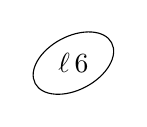
\begin{tikzpicture}[baseline=(t.base)]\node[inner sep=3pt] (t) {$\ell\,6$};\draw[rotate=28] (0,0) ellipse (0.55 and 0.34);\end{tikzpicture}}
une référence ou définition pour réduction semi-stable d'une courbe (seule la terminologie de ``réduction stable'' se trouve dans [3])

iv)\quad $\ell\,12$\quad orthographe ?\qquad \unsure{système}

\figure{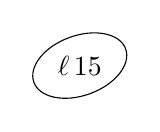
\begin{tikzpicture}[baseline=(t.base)]\node[inner sep=3pt] (t) {$\ell\,15$};\draw[rotate=20] (0,0) ellipse (0.62 and 0.38);\end{tikzpicture}}
vider la Rmq sur les $H^i$ (qui n'est ni
\figure{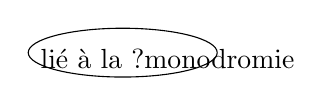
\begin{tikzpicture}[baseline=(t.base)]\node[anchor=west,inner sep=0pt] (t) at (0,0) {lié à la \inserted{?}monodromie};\draw (1.05,0.08) ellipse (1.20 and 0.31);\end{tikzpicture}}, ni fondé sur des théorèmes)

\figure{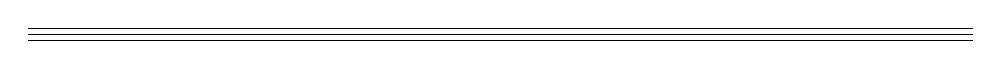
\begin{tikzpicture}\draw (0,0)--(12,0);\draw (0,-0.08)--(12,-0.08);\draw (0,-0.16)--(12,-0.16);\end{tikzpicture}}

1.

\uline{p 0.}\quad titre :\qquad $\ell'$ (minuscule)

$(1.0)\ \ell\,5$\qquad donc\qquad ?

\figure{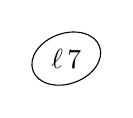
\begin{tikzpicture}[baseline=(t.base)]\node[inner sep=3pt] (t) {$\ell\,7$};\draw[rotate=20] (0,0) ellipse (0.45 and 0.32);\end{tikzpicture}}
à quel concept se rapporte ``lequel''.

\rule{\linewidth}{0.3pt}

\uline{p.1}\quad $\ell\,12$\quad français : choisie\quad ; ``qui est'' tend à faire croire qu'on impose une condition supplémentaire

$\ell\,16$\quad $=B$ donc le symbole est \unsure{malheureux};\quad $=A'_K$ de toute façon.

\rule{\linewidth}{0.3pt}

p2\quad $\ell\,2$\quad pourquoi
\figure{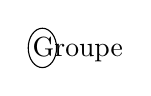
\begin{tikzpicture}[baseline=(t.base)]\node[anchor=west,inner sep=0pt] (t) at (0,0) {Groupe};\draw (0.13,0.02) ellipse (0.18 and 0.25);\end{tikzpicture}}
\quad -- épimorphisme n'est pas la définition d'isogénie --

$\ell\,15$\quad -- supprimer séparé type fini au bénéfice du seul quasi projectif.

-- que $A\mathbin{\underset{S}{\times}}\operatorname{Spec}(K)\xrightarrow{\sim}A_K$ est une trivialité

\margin{2}
